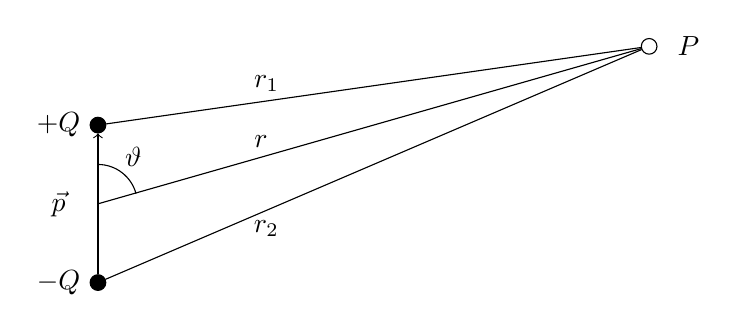
\begin{tikzpicture}
	
	% Styles
	\tikzstyle{dot} = [draw,shape=circle,scale=0.6]
	\tikzstyle{label} = [node distance=5mm]
	\tikzstyle{linelabel} = [pos=0.3,above]

	% Ladungen
	\node at (0,0) [dot,fill=black] (neg) {};
	\node at (0,1) (mom) {};
	\node at (0,2) [dot,fill=black] (pos) {};
	\draw[->] (neg) -- (pos);

	% Labels Ladungen
	\node [label,left of=pos] {$+Q$};
	\node [label,left of=mom] {$\vec{p}$};
	\node [label,left of=neg] {$-Q$};

	% Punkt P mit Verbindungslinien
	\node at (7,3) [dot,fill=white] (P) {};
	\node [label,right of=P] {$P$};
	\draw (pos) -- node [linelabel] {$r_1$} (P);
	\draw (mom.center) -- node [linelabel] {$r$} (P);
	\draw (neg) -- node [linelabel,below] {$r_2$} (P);

	% Winkel
	\draw (0,1.5) arc (90:15:0.5);
	\node at (0.45,1.6) {$\vartheta$};

\end{tikzpicture}
